\section{Flow estimation}
%\subsection{Flow estimation}
\label{sec:core}

The object flow consist on computing the motion field for an object of interest through an image
sequence. The most usual approach to solve a problem like this is to implement some of the available
optical flow techniques through the complete sequence and perform the flow integration. 
However, this process results in high levels of motion drift \cite{c18}\cite{c19} and usually the motion of the interest
object is affected by a global regularization. In some extreme cases, the interest object motion
may be totally blurred and other techniques have to be incorporated. Moreover, the diversity
of natural video sequences makes difficult the choice of one optical flow technique over another, even when specialized
databases are at hand \cite{c17}, because currently no single method can achieve a strong 
performance in every of the available datasets. Most of these methods consist in the minimization 
of an energy function with two terms (As was previously mentioned in the Sec. \ref{chap:intro}). The data
term is mostly shared between different approaches, but the prior or spatial term is different, and basically states 
under what conditions the optical flow smoothness should be maintained or not. In a global approach, however,
this is a difficult concept to define. Most of these smoothness terms rely in appearance differences or gradients.
All these meaning that, unavoidably, some methods may be more reliable for some cases but weaker for others. 
It can be argued that this behaviour may be caused because most of the techniques do not count with a way to identify 
firmly where exactly this smoothness prior can be applied. 

It is difficult, nevertheless, to blame the authors for the choice of some regularization 
terms, since the more robust the regularization terms is, and the higher level knowledge is applied, the more difficult is to minimize the 
energy function, and thus, the more difficult is to obtain a reliable global solution. 
The modern advances in non-convex optimization methods have allowed some authors 
to go further in the writing of these energy functions, but at the end they still rely in the pixel level to determine whether a strong regularization 
should be applied to a zone or not.


   \begin{figure}[thpb]
      \centering
      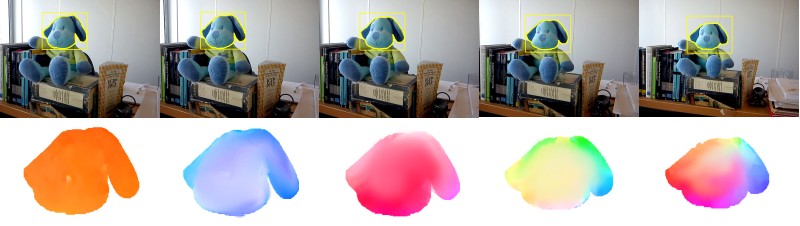
\includegraphics[width=1.0\textwidth]{../images/objectflow.png}
      \caption{Object flow with the color code of \cite{c17} (bottom) for frames in the Puppy sequence (up). }
      \label{of}
   \end{figure}

The main idea behind the object flow is that given the availability of several robust tracking techniques, and the proposed
segmentation method for video, the optical flow computation can be refined by computing it successively between pairs
of tracked windows. The basic proposal to perform this refinement consist on considering the segmentation limits  as reliable smoothness boundaries. 
This is, of course, under the assumption that the motion is indeed smooth within the object region. 
This  assumption is not far from reality in most scenes with an interest object, and it is indeed a better way to determine the limits of the regularization 
than using the difference between raw pixel values.
Naturally, as the object tracker is included, is expected that the object flow should be more robust to rapid motions than the
optical flow. 
Thus, the full motion is split in two, the long range motion, given by the tracker window, and the precision part, given by the targeted optical flow. The Fig. \ref{of} shows 
the object flow for several frames in the Puppy sequence, and the Fig. \ref{of2} shows the same for the MPI\_S1 sequence. Observe the motion vectors are computed 
only inside the object of interest, preserving a strong smoothing prior, but 
also allowing internal variations in the flow. 

   \begin{figure}[thpb]
      \centering
      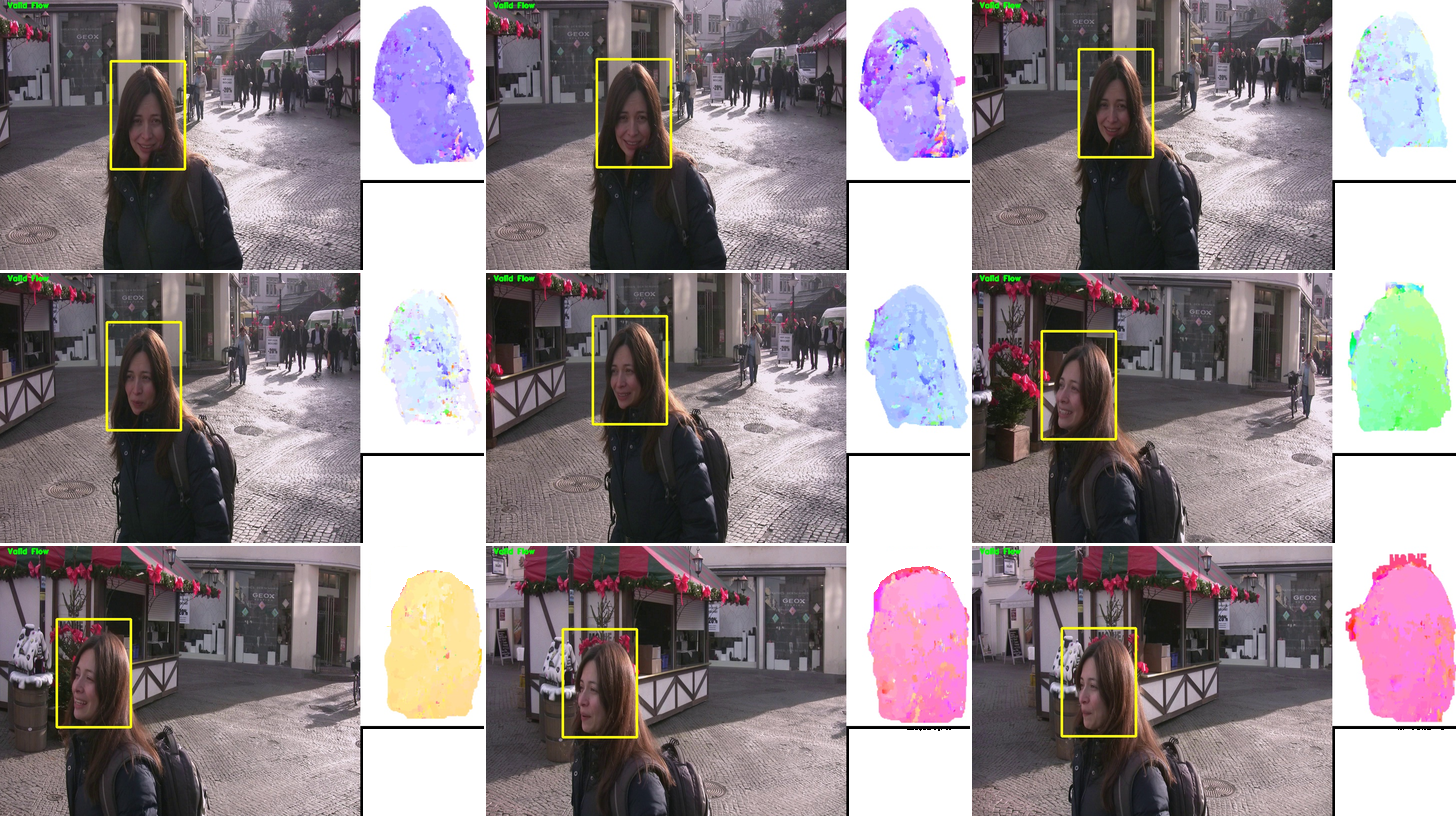
\includegraphics[width=1.0\textwidth]{../images/other_of.png}
      \caption{ Object flow for several frames of the MPI\_S1 sequence. The flow is shown enlarged for better details.}
      \label{of2}
   \end{figure}

As a first approximation to the object flow, the Simple Flow technique \cite{c21} is taken as core base. This is because of its scalability 
to higher resolutions and because its specialization to the concept of object flow is only natural. The reason behind this is that in the Simple Flow pipeline 
the smoothness localization can be easily specified through computation masks. More specifically, the initial computation mask is derived from 
the segmentation performed as prior step. An iterative multi-scale approach based on this initialization follows. The original method uses bilateral filtering to refine each flow result. 
However, as a reliable segmentation mask is provided, this bilateral filtering is replaced by a Gaussian filter applied within the limits of this mask, highly improving the speed of the 
flow estimation. 

   \begin{figure}[thpb]
      \centering
      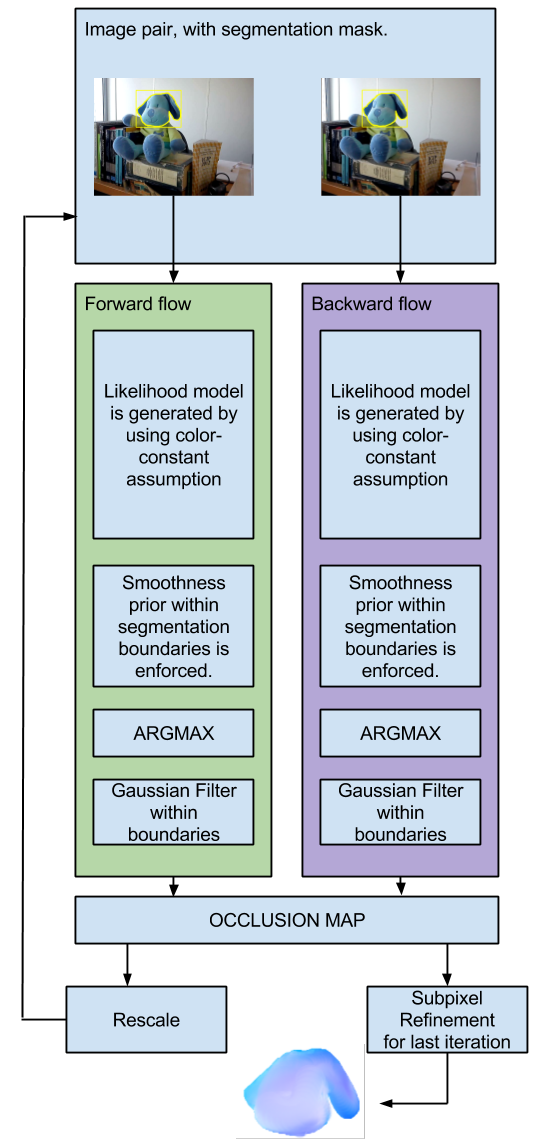
\includegraphics[height=1.0\textheight]{../images/simpleobjectflow.png}
      \caption{ Simple object flow algorithm diagram.}
      \label{sof_d}
   \end{figure}

In more detail, 
for every pixel within the segmentation boundaries a vector $e$ of dimension $n^2$ is computed 
by extracting a color difference $n$x$n$ window centred in that pixel. The energy $E$ (as in \ref{eq_simple}) is computed 
within the 
segmentation boundaries 
by applying a bilateral filter, 
using the color data of the initial 
frame to define the filter weights. 
The flow for the given pixel is the vector that minimizes $E$. The final bilateral filter applied over the computed flow field for every scale is replaced by a Gaussian filter limited by the segmentation masks. The process is done twice, from $I_t$ to $I_{t+1}$ and vice-versa. 
An occlusion mask is generated by eliminating the flows that do not correspond with its 
backward counterpart ($||(u_f,v_f)-(-u_b,-v_b)||$ is too high). The process is repeated in 
several scales to account for possible large motions inside the studied object (Fig. \ref{sof_d}).

However, direct modifications in other optical flow methods can be further studied. For instance, in graph-cut based 
minimization approaches, the regularity constraints can be precisely targeted by disconnecting foreground pixels from background ones.

   \begin{figure}[thpb]
      \centering
      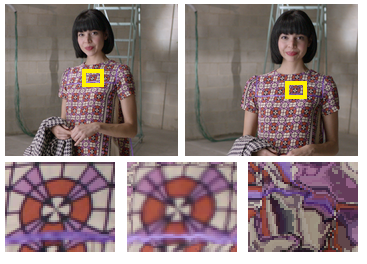
\includegraphics[width=0.66\textwidth]{../images/objectflow_nosegm.png}
      \caption{Top row: First and last frames used from the Amelia sequence. Bottom row: From left to right: Groundtruth patch; patch generated with the 
basic object flow combining the {\it Struck} Tracker and the {\it TVL1} optical flow; and patch generated with the globally computed  {\it TVL1} optical flow.}
      \label{of_nose}
   \end{figure}

The object flow concept is valid, however, for those cases where there is not a separable object, and the segmentation is not valid or possible to extract. 
In order to show this and the fact that only combining the tracker information with a locally computed optical flow is already an improvement to a global 
optical flow, the Fig. \ref{of_nose} shows an experiment where a patch from a dress is extrapolated by using the most basic object flow definition (no segmentation) 
and by a globally computed optical flow. It can be seen that the results are better for the first method.



